\documentclass{article}
%\usepackage{nips_2018}
% The authors do not need to be anonymized for a workshop submission.
\usepackage[final]{nips_2018}

%\usepackage[top=1in,bottom=1in,left=1in,right=1in]{geometry}
\usepackage[utf8]{inputenc}
\usepackage[T1]{fontenc}    % use 8-bit T1 fonts
\usepackage{hyperref}       % hyperlinks
\usepackage{url}            % simple URL typesetting
\usepackage{booktabs}       % professional-quality tables
\usepackage{amsfonts}       % blackboard math symbols
\usepackage{nicefrac}       % compact symbols for 1/2, etc.
\usepackage{microtype}      % microtypography
\usepackage{prettyref}

\usepackage{amsmath}
\usepackage{amssymb}
\usepackage{setspace}
\usepackage{color}
\usepackage{graphicx}
\usepackage{listings}
\usepackage{subcaption}
\usepackage{authblk}

% By including the boilerplate that begins knitr output once, we can
% have \input{} individual knitted files below.
\usepackage[]{graphicx}
\usepackage[]{color}
%% maxwidth is the original width if it is less than linewidth
%% otherwise use linewidth (to make sure the graphics do not exceed the margin)
\makeatletter
\def\maxwidth{ %
  \ifdim\Gin@nat@width>\linewidth
    \linewidth
  \else
    \Gin@nat@width
  \fi
}
\makeatother

\definecolor{fgcolor}{rgb}{0.345, 0.345, 0.345}
\newcommand{\hlnum}[1]{\textcolor[rgb]{0.686,0.059,0.569}{#1}}%
\newcommand{\hlstr}[1]{\textcolor[rgb]{0.192,0.494,0.8}{#1}}%
\newcommand{\hlcom}[1]{\textcolor[rgb]{0.678,0.584,0.686}{\textit{#1}}}%
\newcommand{\hlopt}[1]{\textcolor[rgb]{0,0,0}{#1}}%
\newcommand{\hlstd}[1]{\textcolor[rgb]{0.345,0.345,0.345}{#1}}%
\newcommand{\hlkwa}[1]{\textcolor[rgb]{0.161,0.373,0.58}{\textbf{#1}}}%
\newcommand{\hlkwb}[1]{\textcolor[rgb]{0.69,0.353,0.396}{#1}}%
\newcommand{\hlkwc}[1]{\textcolor[rgb]{0.333,0.667,0.333}{#1}}%
\newcommand{\hlkwd}[1]{\textcolor[rgb]{0.737,0.353,0.396}{\textbf{#1}}}%
\let\hlipl\hlkwb

\usepackage{framed}
\makeatletter
\newenvironment{kframe}{%
 \def\at@end@of@kframe{}%
 \ifinner\ifhmode%
  \def\at@end@of@kframe{\end{minipage}}%
  \begin{minipage}{\columnwidth}%
 \fi\fi%
 \def\FrameCommand##1{\hskip\@totalleftmargin \hskip-\fboxsep
 \colorbox{shadecolor}{##1}\hskip-\fboxsep
     % There is no \\@totalrightmargin, so:
     \hskip-\linewidth \hskip-\@totalleftmargin \hskip\columnwidth}%
 \MakeFramed {\advance\hsize-\width
   \@totalleftmargin\z@ \linewidth\hsize
   \@setminipage}}%
 {\par\unskip\endMakeFramed%
 \at@end@of@kframe}
\makeatother

\definecolor{shadecolor}{rgb}{.97, .97, .97}
\definecolor{messagecolor}{rgb}{0, 0, 0}
\definecolor{warningcolor}{rgb}{1, 0, 1}
\definecolor{errorcolor}{rgb}{1, 0, 0}
\newenvironment{knitrout}{}{} % an empty environment to be redefined in TeX

\usepackage{alltt}


%\usepackage[authoryear]{natbib}
%\usepackage[nonatbib]{nips_2018}

% \setlength{\parskip}{1em}
% \setlength{\parindent}{0pt}

\newcommand{\Rbb}{\mathbb{R}}
\newcommand{\Expect}{\mathbb{E}}
\newcommand{\Var}{\text{Var}}
\newcommand{\Cov}{\text{Cov}}
\DeclareMathOperator*{\argmin}{arg\,min}
\DeclareMathOperator*{\argsup}{arg\,sup}
\DeclareMathOperator*{\arginf}{arg\,inf}
\newcommand{\iid}{\stackrel{iid}{\sim}}
\newcommand{\indep}{\stackrel{indep}{\sim}}
\newcommand{\vbfamily}{\mathcal{Q}}
\newcommand{\etaopt}{\eta^{*}}
\newcommand{\etazopt}{\eta_z^{*}}
\newcommand{\etathetaopt}{\eta_\theta^{*}}
\newcommand{\qopt}{q^{*}}
\newcommand{\targethat}{\hat{g}}
\newcommand{\QExpect}
{\Expect_{q\left(\theta, z \vert \eta_\theta, \etazopt(\eta_\theta)\right)}}
\newcommand{\atzero}{\Big\rvert_{\eta_\theta = \etathetaopt, \epsilon = 0}}
\newcommand{\etathetalin}{\eta_\theta^{LIN}}

\newrefformat{eq}{Equation \ref{#1}}
\newrefformat{app}{Appendix \ref{#1}}


% \DeclareMathOperator*{\sup}{sup}

\title{Evaluating Sensitivity to the Stick Breaking Prior in Bayesian Nonparametrics}

\author[1*]{Runjing (Bryan) Liu}
\author[1*]{Ryan Giordano}
\author[1]{Michael I.~Jordan}
\author[2]{Tamara Broderick}

\affil[*]{These authors contributed equally}
\affil[1]{UC Berkeley}
\affil[2]{MIT}


\begin{document}
\maketitle

\section{Introduction}\label{sec:introduction}

A central question in many probabilistic clustering problems is how many
distinct clusters are present in a particular dataset.
% In all but the simplest
% problems, any attempt to answer this question may be strongly determined by the
% criterion used.
Bayesian nonparametrics (BNP) addresses this question by placing a generative
process on cluster assigment, making the number of distinct clusters present
amenable to Bayesian inference.  However, like all Bayesian approaches, BNP
requires the specification of a prior which may favor a greater or fewer number
of distinct clusters.  In the extreme, there exist prior specifications that
will place the preponderance of posterior mass either on a single cluster or as
many distinct clusters as there are datapoints.  Hopefully, reasonable priors
will lie somewhere in between, with the inferred number of clusters present
being largely determined by the likelihood and data, not the prior.  In
practice, however, it is important to quantitatively establish that the prior is
not too imformative, particularly when---as is often the case in BNP---the
particular form of the prior is chosen for mathematical convenience rather than
because of a considered subjective belief.

We derive sensitivity measures of the expected number of distinct clusters
present for trucated variational Bayes (VB) approximation to a BNP clustering
problem.  Using a stick-breaking represenation of a Dirichlet process, we
consider perturbations both to the scalar concentration parameter and to the
functional form of the stick-breaking distribution.  Unlike previous work on
local Bayesian robustness \citep{gustafson:1996:localposterior,
Basu:2000:BNP_robustness}, we pay special attention to the ability of our
sensitivity measures to \emph{extrapolate} to different priors, rather than
treating the sensitivity as a measure of robustness \textit{per se}.  This
leads us to

We apply our methods to cluster the Iris \citep{iris_data_anderson,
iris_data_fisher} dataset, comparing our results to the much more expensive
process of re-fitting the model.

% A central question in many probabilistic clustering problems is how many
% distinct clusters are present in a particular dataset. In all but the simplest
% problems, any attempt to answer this question may be strongly determined by the
% criterion used. One common approach, based in the Bayesian tradition, addresses
% the problem with a generative model: out of a population of unobserved latent
% clusters, some finite number are randomly chosen to be present in the actual
% data at hand. The identity and number of these clusters can then be estimated –
% with attendant uncertainty estimates – using the tools of Bayesian posterior
% inference. For example, one might estimate the ``number of distinct clusters
% present'' by its posterior expectation. Such a generative model is called a
% ``Bayesian non-parametric'' (BNP) model when the number of latent clusters is
% infinite, though, naturally, even in non-parametric models only a finite number
% of clusters can actually be observed in any particular dataset.
%
% As with any Bayesian model, this approach requires the specification of a prior
% and a likelihood. In this case, the likelihood describes the dispersion of data
% within a particular cluster, and the prior determines both the distribution of
% cluster shapes and sizes as well as the process that determines how many
% clusters are present. In general, different choices of the prior and likelihood
% would give different answers to the question “how many distinct clusters are
% present?” For example, if the prior does not somehow prefer fewer, larger
% clusters, then there is nothing that inherently prevents such an approach from
% inferring that each datapoint is in its own cluster. However, one still hopes
% that a broad range of reasonable choices of prior and likelihood will come to
% similar conclusions. Consequently it is important, in practice, to measure the
% sensitivity of the inferred number of clusters present to the prior and
% likelihood specification. Furthermore, these sensitivity measures should work
% with the kinds of inference tools that are used in practice, operate relatively
% automatically without re-fitting the model many times, and measure sensitivity
% not only to alternative hyperparameters but also to alternative functional forms
% of the prior and likelihood.
%
% To address these needs, we develop fast, automatic measures of the sensitivity
% of variational Bayes (VB) approximations to perturbations of functional forms in
% a putative model. As a motivating application, we apply our techniques to
% estimate the sensitivity of BNP posteriors to the functional form of a
% particular BNP prior known as the stick-breaking prior. Stick-breaking priors
% provide a strong motivation to quantify functional perturbations. A typical
% choice of a stick breaking prior is specified with only a single real-valued
% hyperparameter and also a potentially informative distributional assumption, the
% form of a stick breaking prior can substantially inform the number of clusters
% inferred to be present in a particular dataset, and it is arguably difficult for
% ordinary practitioners to form meaningful subjective beliefs about the abstract
% form of the stick breaking prior.

% We begin by deriving a general result for the sensitivity of VB optima to
% function-valued perturbations, as well as several useful specializations. We
% then describe a VB approximation to a BNP model with a stick-breaking prior and
% derive the sensitivity of the approximate number of inferred clusters to the
% choice of the stick breaking prior. We then apply our methods to cluster the
% Iris \citep{iris_data_anderson, iris_data_fisher} dataset, comparing our results
% to the much more expensive process of re-fitting the model.


\section{Model and Inference}\label{sec:model}
\paragraph{Data and model.}
We use the Iris dataset \citep{iris_data_anderson, iris_data_fisher}, which
contains 150 observations of three different types of iris flowers. We use
measurements of their sepal length, sepal width, petal length, and petal width
to cluster the data with the goal of recovering the three species. Let $y_{n}\in
\mathbb{R}^4$ be these four measurements for flower $n$.

In the spirit of BNP, let us suppose that there there are an infinte number of
distinct species of iris in the world, indexed by $k=1,2,3,\ldots$, only some
finite number of which are present in our observed dataset.  Let $z_n$ denote
the index of the cluster (i.e. the species) to which flower $n$ belongs, i.e.,
$z_n = k$ for exactly one $k$. Each cluster has mean $\mu_k\in
\mathbb{R}^4$ and covariance $\Sigma_k \in \mathbb{R}^{4\times 4}$, and we write
the collections as $\mu = \left(\mu_1, \mu_2, ...\right)$ and $\Sigma =
\left(\Sigma_1, \Sigma_2, ... \right)$. Our data-generating process given the
model parameters is then
%
\begin{align*}
	y_n | z_n, \mu, \Sigma \sim
        \mathcal{N}\left(
            y_n \Big\vert
                \sum_{k=1}^\infty \mathbb{I}\{z_n = k\} \mu_k \;,
              \; \sum_{k=1}^\infty \mathbb{I}\{z_n = k\} \Sigma_k\right),
	\quad n = 1, ..., N.
\end{align*}
%
For $\mu$ and $\Sigma$, we use dispersed IID conjugate priors. For the prior on
the cluster memberships $z_n$, we use a stick breaking representation of a BNP
Dirichlet process prior \citep{ferguson:1973:bayesian,
sethuraman:1994:constructivedp}. Specifically, we define latent stick lengths
$\nu=\left(\nu_1, \nu_2, ...\right)$, a concentration parameter $\alpha>0$, and
base stick-breaking distribution $p_{0}\left(\nu_k \vert \alpha \right) =
\mathrm{Beta}\left(\nu_k \Big\vert 1, \alpha \right)$.  The prior on the cluster
assignments $z_n$ for $n=1,...,150$ is then given by
%
\begin{align}
\nu \vert \alpha \sim \prod_{k=1}^\infty p_{0}\left(\nu_k \vert \alpha \right)
\textrm{,}
    \quad\textrm{ with }\quad
\pi_k | \nu := \nu_k \prod_{j=1}^{k-1} (1 - \nu_j)
\quad\textrm{ and }\quad
z_n \vert \pi \iid \mathrm{Categorical}(\pi). \label{eq:stick_breaking}
\end{align}
%
The concentration parameter $\alpha$ and stick-breaking prior $p_{0}$
thus determine our prior belief about the number of clusters present.
We will be examining the sensitivity of our posterior beliefs about the
number of clusters present to our choice for $\alpha$ and $p_{0}$.


%\section{Variational approximation}\label{sec:variational_approx}
%
\paragraph{Variational approximation.}
It is difficult to calculate the posterior $p\left(\nu, \mu, \Sigma, z \vert
y\right)$, both because the normalizing constant is intractable and because
$K=\infty$ in a true BNP representation. In order to perform approximate
inference, we use a truncated VB approximation
\citep{blei:2006:dirichletbnp}. For compactness of notation, let $\theta =
\left(\nu, \mu, \Sigma\right)$ denote the collection of ``global'' parameters,
i.e., parameters whose values affect the data-generating process of every
observation $y_n$.   Let $\delta\left(\cdot\right)$ denote a delta function. We
define a class of approximating distributions for VB as
%
\begin{align*}
\vbfamily := \Big\{ q:
q(\theta, z) &=
\left(\prod_{k=1}^{K}q\left(\nu_{k}\right)\delta\left(\mu_{k}\right)
    \delta\left(\Sigma_{k}\right)\right)
    \left(\prod_{n=1}^{150}q\left(z_{n}\right) \right)\textrm{, where } \\
q\left(\nu_{k}\right) &= \mathrm{Lognormal}\left(\nu_k\right) \textrm{ and }
q\left(z_n\right) = \mathrm{Categorical}\left(z_n\right)
\Big\}.
\end{align*}
%
The family $\vbfamily$ is parameterized by a finite-dimensional vector containing
the locations of the delta functions and the parameters for the lognormal
distributions,
%
\footnote{We use the lognormal distribution rather than the conjugate Beta
distribution because the lognormal makes numerical integration easier when
re-optimizing using non-conjugate $p_{0k}$.  Were one to simply rely on our
sensitivity measures and not re-optimize, there would be no need for numerical
integration, and the more convenient Beta variational approximation could be
used.}
%
which we denote by $\eta_\theta$, and the parameters for the
multinomial distributions, which we denote by $\eta_z$. We write the combined
parameters as $\eta=\left(\eta_\theta, \eta_z\right)$. That is, $\eta$ is
defined such that
%
$\vbfamily =
    \left\{q: q\left(\theta, z\right) =
            q\left(\theta, z \vert \eta \right) =
            q\left(\theta \vert \eta_\theta \right)
            q\left(z \vert \eta_z \right)
    \right\}.$
%
The variational approximation is then given by
%
%\begin{align*}
$
\etaopt = \argmin_{\eta} KL\left(
    q(\theta, z \vert \eta) \big\| p(\theta, z | y)
    \right). %\label{eq:kl_objective}
$
%\end{align*}
%
%Let $\qopt\left(\theta, z\right) = q\left(\theta, z \vert \etaopt\right)$.

It will be important later to note that it is easy to calculate the optimal
$\eta_z$ for a given $\eta_\theta$ because the model is conditionally conjugate,
i.e., $p\left(z \vert \theta, y\right)$ is categorical, and so is $q\left(z
\vert \eta_z\right)$.  Specifically, there exists an easily-calculated, closed
form for
%
%\begin{align}
$
\etazopt\left(\eta_\theta\right) = \argmin_{\eta_z}
    KL\left(
    q(\theta \vert \eta_\theta) q( z \vert \eta_z)
        \big\| p(\theta, z | y)
    \right).
$
%\label{eq:z_update}
%\end{align}
%

%%%%%%%%%%%%%%%%
%%%%%%%%%%%%%%%%
%%%%%%%%%%%%%%%%


\paragraph{Target posterior quantity.}

We are interested in the inferred number of clusters present in the observed
data, which can be expressed as an expection with respect to
$q\left(z \vert \eta_z \right)$, and therefore as a function of
$\etathetaopt$ via the relation $\etazopt(\eta_\theta)$:
%
\begin{align}
g(\etathetaopt) &:=
\Expect_{q(\theta, z \vert \etaopt)} \left[ \#\{\text{distinct clusters}\} \right]  =
\Expect_{q(z \vert \etazopt(\eta_\theta))} \left[
    \sum_{k=1}^K \left(1 - \prod_{n=1}^N \mathbb{I}\{z_n \ne k\} \right) \right].
    \label{eq:expected_num_clusters}
\end{align}
%
For a given optimal set of global variational parameters,
$g(\etathetaopt)$ can be computed with Monte-Carlo draws of the cluster
indicators,
$z \iid q\left(z \vert \etazopt(\etathetaopt)\right)$.


\section{Hyper-parameter sensitivity}\label{sec:hyper_param_sens}

\paragraph{General hyperparamter sensitivity.}
%
We with to approximate the sensitity of $g(\etaopt)$ to perturbations of the
value of $\alpha$ and to the functional form of $p_{0k}$.  To do this, we will
call on a general result for the sensitivity of VB optima to vectors of
real-valued hyperparameters.  Suppose the exact posterior is parameterized by a
real-valued hyperparameter $\epsilon$, i.e., the posterior is given by
$p\left(\theta, z \vert y, \epsilon\right)$. In the present work, $\epsilon$
will parameterize perturbations to the prior, as we will describe in more detail
shortly.  Then the optimal variational approximation is also a function of
$\epsilon$ through \prettyref{eq:kl_objective}.  We can define
%
\begin{align}
KL\left(\eta_\theta, \epsilon\right) &:=
    KL\left(q(\theta, z \vert \eta_\theta, \etazopt\left(\eta_\theta\right))
    \big\| p(\theta, z | y, \epsilon) \right) \\
\etathetaopt\left(\epsilon\right) &=
    \argmin_{\eta_\theta} KL\left(\eta_\theta, \epsilon\right)
    \label{eq:pert_kl_objective}
\end{align}
%
In general, the dependence of $\etathetaopt\left(\epsilon\right)$ on $\epsilon$ is
complex and non-linear, but we may approximate it with a first-order Taylor
series.
Under mild regularity conditions that are satisfied in the present case,
\citet[Theorem 2]{giordano:2017:covariances} gives a closed form
expression for this Taylor series.
Without loss of generality, let $\epsilon=0$ represent the unperturbed
posterior, so that $p\left(\theta, z \vert y, \epsilon=0\right) = p\left(\theta,
z \vert y \right)$.
Define
$H := \partial^2 KL(\eta_\theta, \epsilon) /
    \partial \eta_\theta \partial \eta_\theta^T
    \atzero$ and
$f_\eta := \partial^2
    \QExpect \left[ \log p\left(y, \theta, z \vert \epsilon \right) \right]
    / \partial \eta_\theta \partial \epsilon^T
    \atzero$.
Then
%
\begin{align}
\etathetaopt(\epsilon)  -  \etathetaopt(0) &\approx
\frac{d \etathetaopt(\epsilon)}{d\epsilon^T}\Big|_{\epsilon=0} \epsilon =
- H^{-1} f_\eta \epsilon
\label{eq:our_approximation}
\end{align}
%
Note that $H$ and $f_\eta$ can be easily evaluated using automatic
differentiation without any need to re-optimize for different $\epsilon$
\citep{maclaurin:2015:autograd} (see \prettyref{app:sensitivity}).  Furthermore,
the Hessian $H$ need be factorized (e.g. with a Cholesky decomposition) or
inverted only once and then re-used to approximate $\etathetaopt(\epsilon)$ for
many different perturbations.

\paragraph{Sensitivity to $\alpha$.}
%
Let $\alpha_0$ be a base value of $\alpha$ at which we optimize for
$\etaopt$. By taking $\epsilon = \alpha - \alpha_0$, and
%
\begin{align*}
f^\alpha_\eta := \frac{\partial^2
    \QExpect
        \left[ \log p\left(\nu \vert \alpha \right) \right]}
{ \partial \eta_\theta \partial \alpha^T }
    \Big\rvert_{\eta_\theta = \etathetaopt, \alpha = \alpha_0},
\end{align*}
%
we can approximate, using Equation \ref{eq:our_approximation},
%
\begin{align*}
\etathetalin(\alpha) := \etathetaopt -
  H^{-1} f^\alpha_\eta (\alpha - \alpha_0) \approx \etathetaopt(\alpha).
\end{align*}
%
We can then approximate
$g\left(\etathetaopt(\alpha)\right) \approx g\left(\etathetalin(\alpha)\right)$.



\paragraph{Functional perturbations.}
%
In order to measure sensitivity to changing the functional form of the prior on
the sticks, we define a parametrized class of multiplicative perturbations to
the base density $p_{0k}$ and apply \prettyref{eq:our_approximation}.
Specifically, fix a multiplicative perturbation $\phi(\cdot): [0, 1] \rightarrow
(0, \infty)$  (recall that the stick lengths $\nu_k\in[0, 1]$), fix
some $\delta\in[0, 1]$, and define
a $\delta$-contaminated prior $p^c_{k}$ on the $k$-th stick by
%
\begin{align}
\label{eq:expon_perturb}
	p^c_{k}(\nu_k ; \delta, \phi) :=
  \frac{p_{0k}(\nu_k)\phi(\nu_k)^\delta}
       {\int_0^1 p_0(\nu_k')\phi(\nu_k')^\delta d\nu_k'}
\end{align}
%
$p^c_{k}$ is defined so that $\delta\in[0, 1]$ interpolates multiplicatively
between the original prior, $p_{0k}$, and a prior proportional to
$\phi(\nu_k)p_{0k}$. For example, we might consider a different prior for the
sticks, say $p_1(\nu_k)$; letting $\phi(\nu_k) = p_1(\nu_k) / p_{0k}(\nu_k)$, we
swap the original prior for the new prior by taking $\delta \rightarrow 1$.

For a fixed $\phi$, we can use \prettyref{eq:our_approximation} by taking
$\epsilon = \delta$ and
%
\begin{align*}
f^{\delta,\phi}_\eta :=
\frac{\partial^2
    \QExpect \left[ \log p^c_{k}(\nu_k ; \delta, \phi) \right]}
{\partial \eta_\theta \partial \delta}
    \Big\rvert_{\eta_\theta = \etathetaopt, \delta = 0} =
\frac{\partial
    \QExpect \left[ \log\phi(\nu_k) \right]}
{\partial \eta_\theta}
    \Big\rvert_{\eta_\theta = \etathetaopt}
\end{align*}
%
Because we have used a multiplicative perturbation, $f^{\delta,\phi}_\eta$
is linear in $\delta$
%
\footnote{Indeed, for the purposes of extrapolating to different priors, this
fact appears to recommend multiplicative perturbations amongst the class of
non-linear perturbations considered by \citet{gustafson:1996:localposterior}.}


% Here,
% %
% \begin{align}
%   \frac{\partial}{\partial \delta} \log p_k^k(\nu_k | \delta, \phi) := \log \phi(\nu_k) -
%     \frac{\int p_0(\nu_k')\log\phi(\nu_k')e^{\delta\phi(\nu_k')} \lambda(d\nu_k')}{\int p_0(\nu_k')\phi(\nu_k')^\delta \lambda(d\nu_k')}
% \end{align}
% %
% The second term does not depend on $\nu_k$, so $f_\eta =
% \frac{\partial}{\partial \eta} E_{q_\eta}[\log \phi(\nu_k)]$.
%
% Now if we perturb each stick $k$ by the same perturbation $\phi(\cdot)$, then
% the derivative of $\eta^*$ with respect to this perturbation is given by
% %
% \begin{align}
%    \frac{d}{d\delta}\eta^*(\delta) &=
%    H^{-1}\frac{\partial}{\partial \eta} E_{q_\eta}\Big[\sum_{k = 1}^K \log \phi(\nu_k)\Big]
%   \label{eq:sensitivity_exp_pert}
% \end{align}
% %
% so derivative for pertubing all the sticks is given by the sum of the deriatives
% of perturbing each stick individually
% \citep{gustafson:2012:localrobustnessbook}.


% \section{Prior work}\label{sec:prior_work}
% %
Our approach has similarities to \citet{Basu:2000:BNP_robustness} who also
considers local robustness in Bayesian non-parametric models. They derive the
analytic derivative of some posterior quantity with respect to the DP prior
parameter $\alpha$. MCMC samples are then needed to evaluate the derivative.
They also consider the robustness with respect to the functional form of the
prior on the cluster means.  By viewing a posterior quantity as a functional of
the functional form of the prior, they evalaute Gateaux derivatives in various
directions to other priors.

In our approach, we analyze the sensitivity of the variational distribution, and
compute derivatives automatically from the KL objective. Moreover, we use the
derivatives not only for sensitivity, but for extrapolating posterior quantities
as they vary over prior parameters.



\section{Results}\label{sec:results}
%%%%%%%%%%%%%%%%%%%%%%%%%%%%%%%%%%%%%%
%%%%%%%%%%%%%%%%%%%%%%%%%%%%%%%%%%%%%%
% Do not edit the TeX file your work
% will be overwritten.  Edit the RnW
% file instead.
%%%%%%%%%%%%%%%%%%%%%%%%%%%%%%%%%%%%%%
%%%%%%%%%%%%%%%%%%%%%%%%%%%%%%%%%%%%%%




% TODO: define these in knitr instead.
\global\long\def\splinedegree{3}
\global\long\def\ntime{14}
\global\long\def\ngenes{1000}
\global\long\def\nclusters{18}
\global\long\def\fullparamdim{66199}
\global\long\def\covregularization{0.1}

\global\long\def\regmat{X_{df}}
\global\long\def\mbe{\mathbb{E}}
\global\long\def\cov{\mathrm{Cov}}
\global\long\def\thetareg{\theta_{r}}
\global\long\def\thetaclust{\theta_{c}}

We start with some DP prior parameter $\alpha_0$. After choosing a different
$\alpha$, we compare the posterior expected number of clusters (
\prettyref{eq:expected_num_clusters}) predicted by our linear approximation
against the expectation obtained from re-optimizing the objective. The results
are shown in \prettyref{fig:parametric_sens_e_num_clusters}.

More specifically, we evaluated the expected number of clusters for a range of
$\alpha$ between 0.5 and 6.5. Then we chose three $\alpha_0$ values, 2, 3.5, and
5, and constructed the linear approximation centered at each of these
$\alpha_0$s. The linear approximation did quite well for choices of $\alpha$
close to $\alpha_0$. Hence, by evaluating the objective at three $\alpha_0$s, we
can use the linear approximation to understand the effect of the DP prior
parameter $\alpha$ across the entire range from 0.5 - 6.5.


\begin{knitrout}
\definecolor{shadecolor}{rgb}{0.969, 0.969, 0.969}\color{fgcolor}\begin{figure}[!h]

{\centering 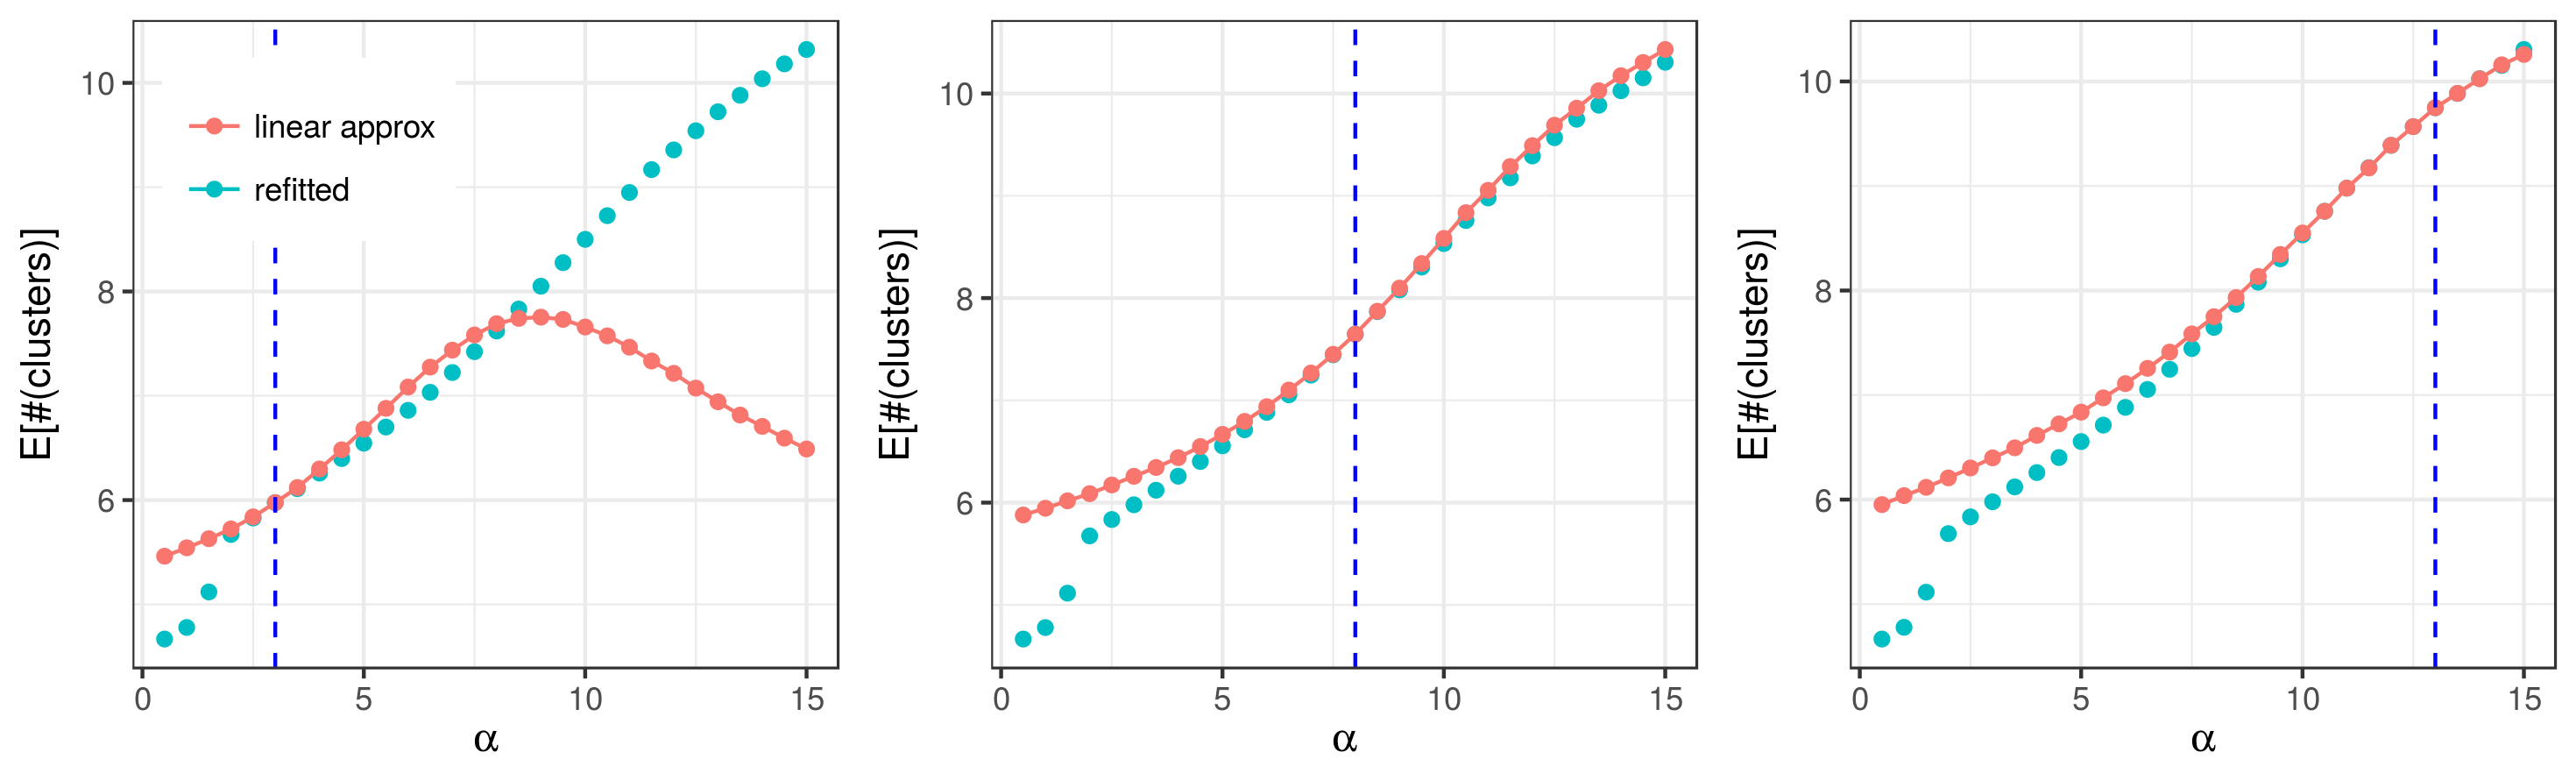
\includegraphics[width=0.98\linewidth,height=0.343\linewidth]{figure/parametric_sens_plot-1} 

}

\caption{\label{fig:parametric_sens_e_num_clusters}Comparison of the expected number of clusters computed by re-optimizing
  the variational objective for various epsilon perturbations to the BNP prior parameter
  (green),
  versus the predicted value from our linear approximation (orange), with alpha0 the
  blue horizontal line.}\label{fig:parametric_sens_plot}
\end{figure}


\end{knitrout}


\subsection{Functional perturbations}
%
We now use the functional perturbation described in
\prettyref{eq:expon_perturb} to perturb the prior on the stick distribution. The
results are shown in \prettyref{fig:func_sens_e_num_clusters}.

We chose two different functional perturbations: for the first we let
$p_1(\nu_k)$ be a logit normal with parameters $\mu = -2, \sigma = 1$; for the
second, we let $p_1(\nu_k)$ be a logit normal with parameters $\mu = 2, \sigma =
1$. In both cases, we then chose $\phi(\nu_k) = p_1(\nu_k) / p_{0k}(\nu_k)$.



\begin{knitrout}
\definecolor{shadecolor}{rgb}{0.969, 0.969, 0.969}\color{fgcolor}\begin{figure}[!h]

{\centering 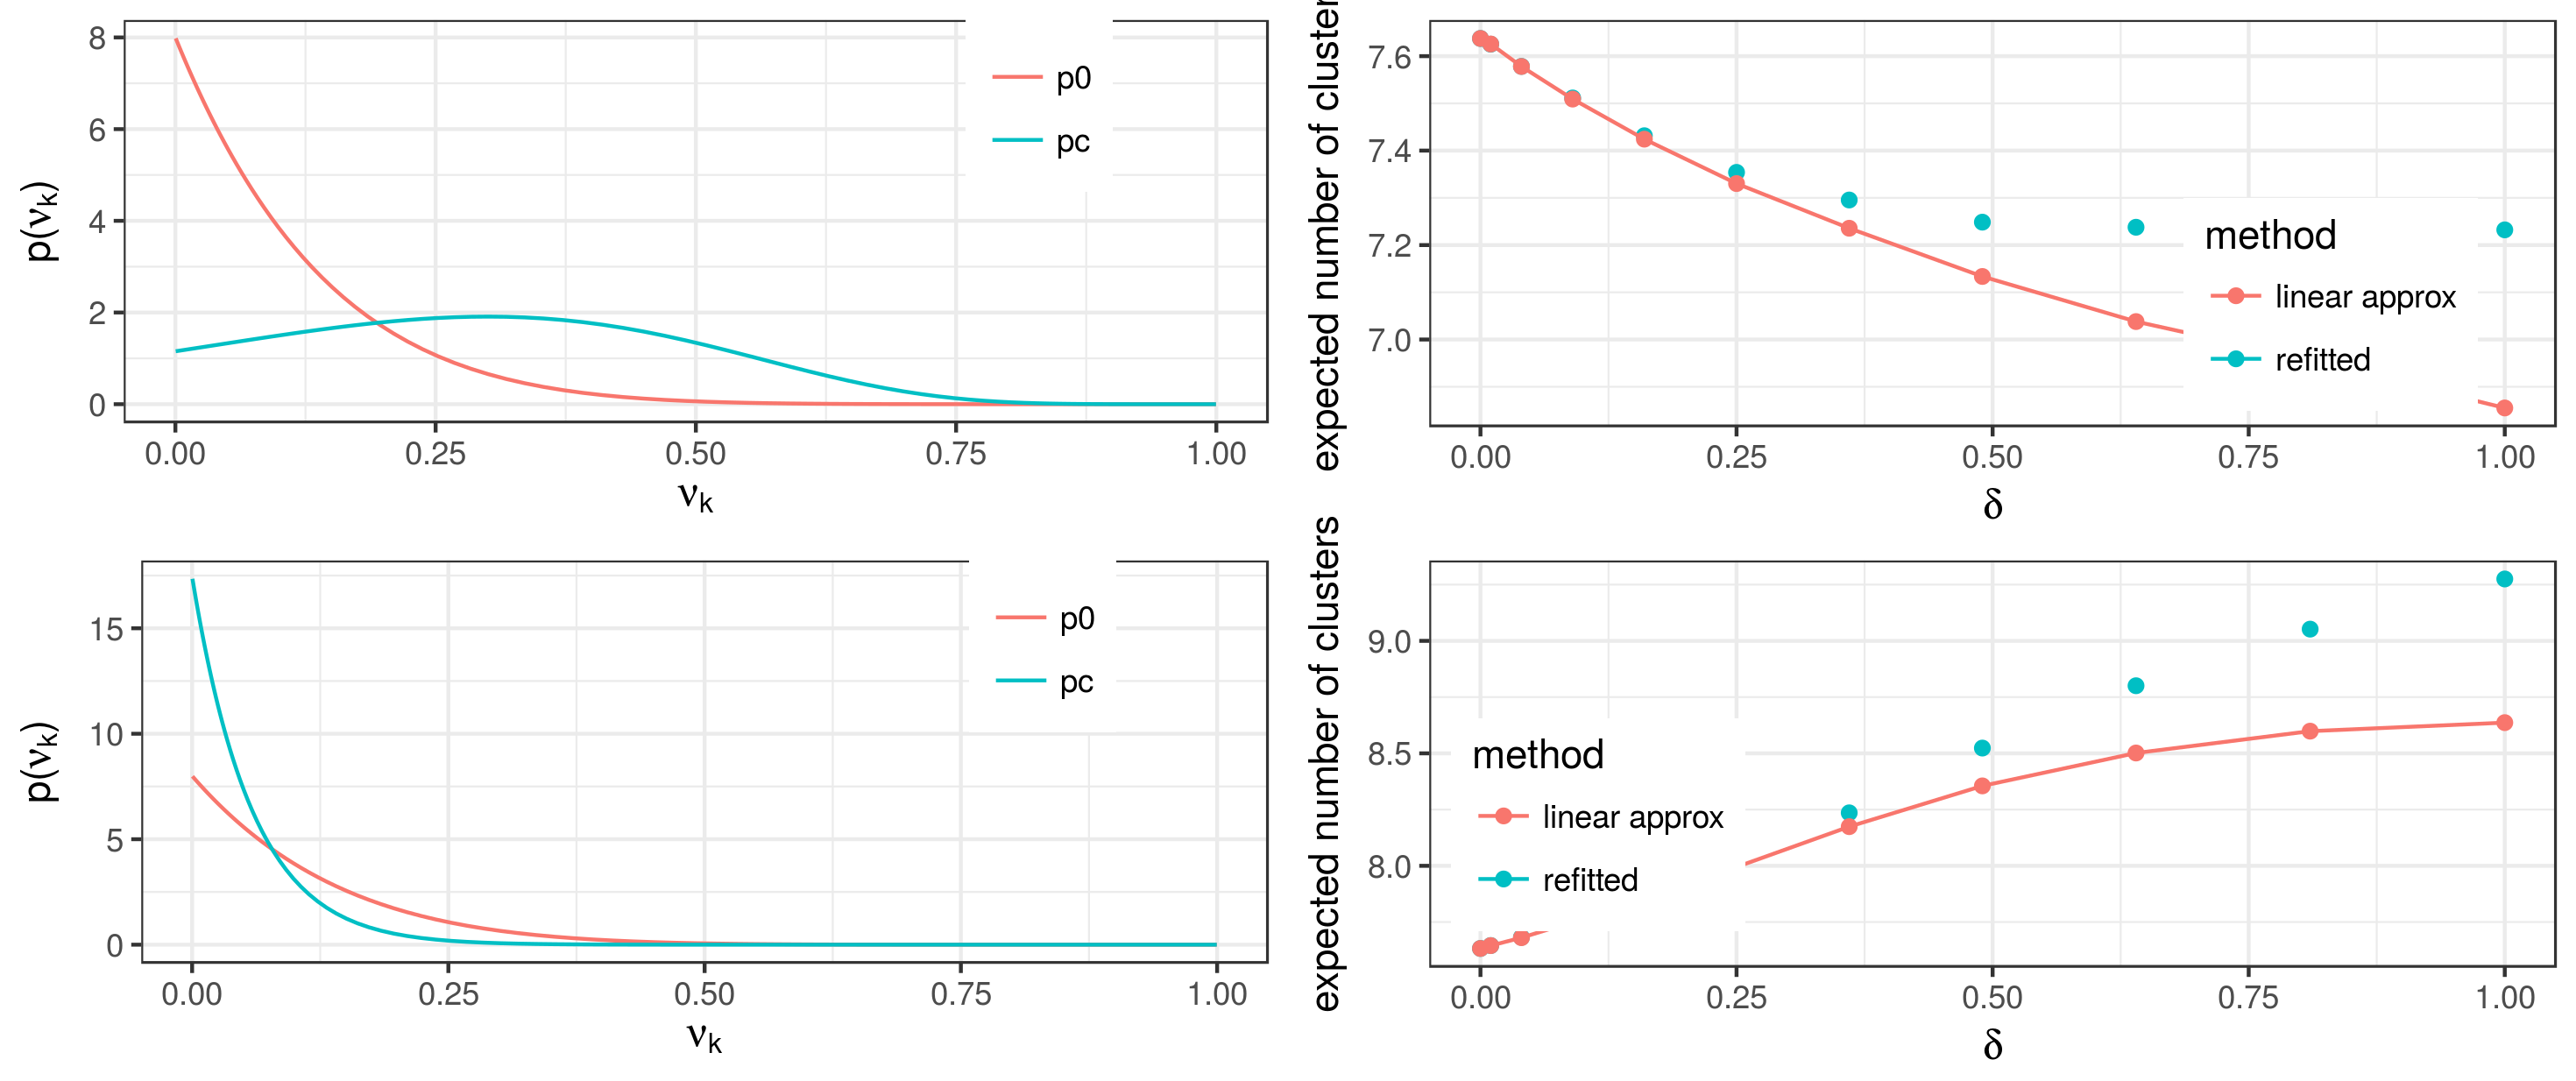
\includegraphics[width=0.98\linewidth,height=0.686\linewidth]{figure/functional_sens_plot-1} 

}

\caption{\label{fig:func_sens_e_num_clusters}
Left column: the original prior p0 in purple, the perturbed prior pc in red. Right: linearly approximated vs.
re-fitted expected number of clusters after the purtubation.  }\label{fig:functional_sens_plot}
\end{figure}


\end{knitrout}



% \begin{figure}[h!]
% 	\centering
% 	\begin{subfigure}[t]{0.32\textwidth}
% 		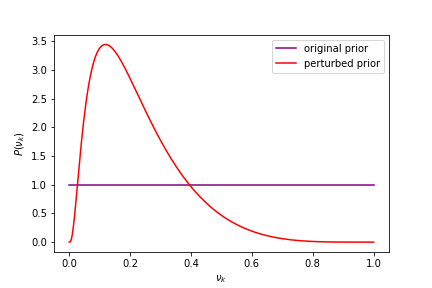
\includegraphics[width = \textwidth]{./functional_sens_results/perturbed_prior1_init3_5.png}
% 		\subcaption{}
% 	\end{subfigure}
%   \begin{subfigure}[t]{0.32\textwidth}
%     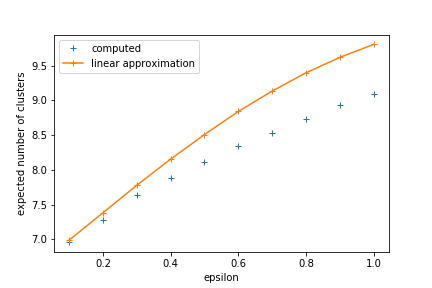
\includegraphics[width = \textwidth]{./functional_sens_results/pred_num_clusters1_init3_5.png}
%     \subcaption{}
%   \end{subfigure}\\
%   \centering
%   \begin{subfigure}[t]{0.32\textwidth}
%     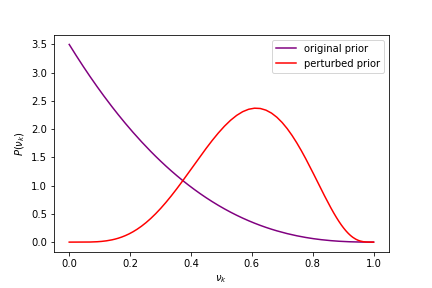
\includegraphics[width = \textwidth]{./functional_sens_results/perturbed_prior2_init3_5.png}
%     \subcaption{}
%   \end{subfigure}
%   \begin{subfigure}[t]{0.32\textwidth}
%     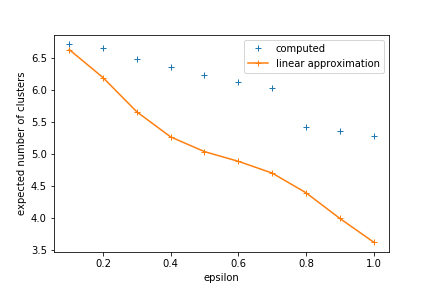
\includegraphics[width = \textwidth]{./functional_sens_results/pred_num_clusters2_init3_5.png}
%     \subcaption{}
%   \end{subfigure}
% 	\caption{Left column: the original prior in purple, the perturbed prior $p_1$ in red. Right: linearly approximated vs.
%   re-fitted expected number of clusters after purturbing each stick by $\phi(\nu_k)^\epsilon =
%   [p_1(\nu_k) / p_{0k}(\nu_k)]^\epsilon$.  }
% 	\label{fig:func_sens_e_num_clusters}
% \end{figure}
%
We find that the linear approximation in this case was able to capture the
direction of the perturbation, (expected number of clusters increased under the
first pertubation, decreased under the second), but did not provide a good
approximation at $\epsilon = 1$.


% \section{Discussion}\label{sec:discussion}
% %
In this work, we fit a BNP model to cluster the Iris dataset, and investigated
the sensitivity of the expected number of posterior clusters to the choice of
stick-breaking prior. We proposed an approximate method that leverages automatic
differentiation tools to efficiently predict the effect of choosing different
stick-breaking priors. We show that for several types of prior perturbations, we
were able to provide a reasonable alternative to the expensive process of
re-fitting a variational posterior.


\newpage
\bibliography{references}
\bibliographystyle{plainnat}

\newpage
\appendix
\section*{Appendices}
%
%
% \section{Calculating the derivative}\label{app:sensitivity}
%
% \citet[Theorem 2]{giordano:2017:covariances} give
% the following expression for
% the derivative $d \etaopt(\epsilon)/ d\epsilon^T \vert_{\epsilon = 0}:$
% %
% \begin{align}
% H &= \frac{\partial^2 KL(\eta, \epsilon)}{\partial \eta \partial \eta^T}
%     \Big\rvert_{\eta = \etaopt, \epsilon = 0} \nonumber \\
% f_\eta &= \frac{\partial^2
%     \Expect_{q\left(\theta, z \vert \eta\right)}
%         \left[ \log p\left(y, \theta, z \vert \epsilon \right)\right]
%     } {\partial \eta \partial \epsilon^T}
%     \Big\rvert_{\eta = \etaopt, \epsilon = 0}  \nonumber  \\
% \frac{d \etaopt(\epsilon)}{d\epsilon^T}\Big|_{\epsilon=0} &=
%     H^{-1} f_\eta. \label{eq:vb_sensitivty}
% \end{align}
% %
% Both $H$ and $f_\eta$ can be evaluated using only $\etaopt(0)$, allowing us to
% use \prettyref{eq:our_approximation} to approximate $\eta$ without re-optimizing
% \prettyref{eq:pert_kl_objective} for different $\epsilon$. Furthermore, $H$ and
% $f_\eta$ can be quickly computed with auto-differentiation tools
% \citep{maclaurin:2015:autograd}. The derivatives and Cholesky factorization of
% $H$ also only need to be computed once, and these calculates can be reused to
% approximate many values of the variational parameters under different
% values of $\epsilon$.


\end{document}
